\documentclass[12pt,a4paper]{article}
\usepackage[margin=0.5in]{geometry}  
\title{數學思通}                          
\author{Ling-Hao Lin}                        
\date{}                               
\usepackage{xeCJK}                   
\setCJKmainfont{標楷體}               
\usepackage{amsthm,amssymb,amsmath}  
\usepackage{enumitem}
\usepackage{derivative}                 

\newtheorem*{theorem}{Theorem}
\newtheorem*{problem}{Problem}         

\usepackage{graphicx}                 %使用插入圖片套件
\usepackage{float}                    %使圖片跟著文章接續,不使圖片跑到頁頭

\xeCJKsetup{CJKmath}                  %使數學式裡可以打中文字

\begin{document}
\maketitle

\begin{theorem}[SIR model]

\begin{align*}
\odv{S}{t}&= -\beta SI \\
\quad\\
\odv{I}{t}&= \beta SI-\gamma\\
\quad\\
\odv{R}{t}&= \gamma I\\
\quad
\end{align*}

\begin{itemize}
\item[S]: the susceptibles who are capable of catching the disease and becoming infected.
\item[I]: the infectives who have the disease and can transmit it.
\item[R]: the removed class consisting of the individuals who are recovered with immunity or dead due to the disease.
\item[$\beta$]: the infection transmission rate.
\item[$\gamma$]: the rate of recovery.
\item[N]: total population, $N=S+I+R$.
\end{itemize}

\end{theorem}
\quad
\begin{problem}[鑽石公主號、2003香港SARS求感染率]

\begin{align*}
\odv{S}{t}\cong \frac{\Delta S}{\Delta t}&=\Delta S\\
\quad\\
                                         &=S_{t+1}-S_{t}=-\beta_{t}S_{t}I_{t}\\
                                         \quad\\
                                         &\Rightarrow \beta_{t}=\frac{S_{t}-S_{t+1}}{S_{t}I_{t}}\\
                                         \quad
\end{align*}

$S_{t}=N-I_{t}-R_{t}$.

\end{problem}

\newpage

\begin{problem}[$R_{0}$, basic reproduction number]
$$R_{0}=\frac{\beta N}{\gamma}$$
\quad
設平均$T$天病毒傳播出去,$N$天後之累積病例數為$R_{0}$之等比級數:
$$1+R_{0}+R_{0}^2+...+R_{0}^n=\frac{R_{0}^{n+1}-1}{R_{0}-1},$$
$n=\frac{N}{T}.$
\end{problem}
\quad
\begin{problem}[Logistic curve fitting idea]

\begin{align*}
\odv{IC}{t}&=\beta_{t}S_{t}I_{t}\\
\quad\\
		   &=\beta_{t}(N-I{t}-R_{t})I_{t}\\
		   \quad\\
		   &=\beta_{t}N(1-\frac{IC_{t}}{N})I_{t}\\
		   \quad\\
		   &\Rightarrow IC_{t}=\frac{N}{1+(N-1)e^{-\beta_{t}Nt}},\\
		   \quad
\end{align*}
$IC_{t}=I_{t}+R_{t}.$
\end{problem}

\begin{figure}[H]                        %使圖片接續文章
\centering                               %將圖片置中
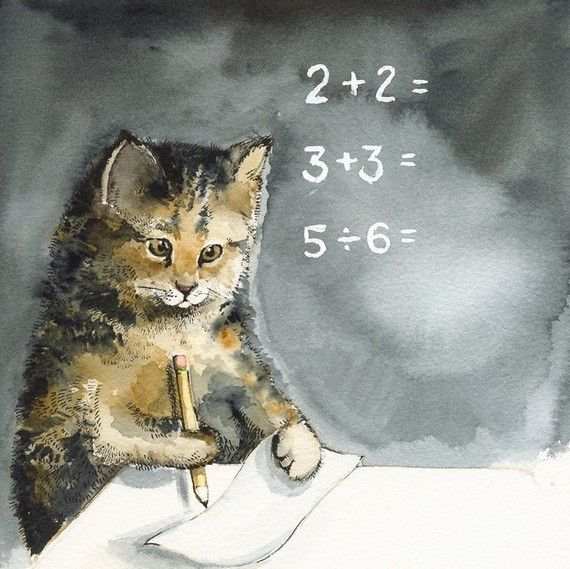
\includegraphics[scale=0.45]{數學貓貓.jpg}
\end{figure}



\end{document}